\providecommand{\main}{../../../..}
\documentclass[\main/dresen_thesis.tex]{subfiles}
\renewcommand{\thisPath}{\main/chapters/theoreticalBackground/ferrites/cobaltferrite}
\begin{document}
  Bulk cobalt ferrite (\ch{CoFe2O4}) is a ferrimagnetic material with a high cubic magnetocrystalline anisotropy and moderate saturation magnetization.
  Due to its high thermal/chemical stability, magnetic properties and cheap production costs, it is of interest for practical use \textit{i.e.} in high-density magnetic recording \cite{Wu_2014_Monol}, magneto-optics \cite{Jung_2005_CoFe2} or spintronics \cite{Ramos_2007_Roomt}.

  \begin{figure}[tb]
    \centering
    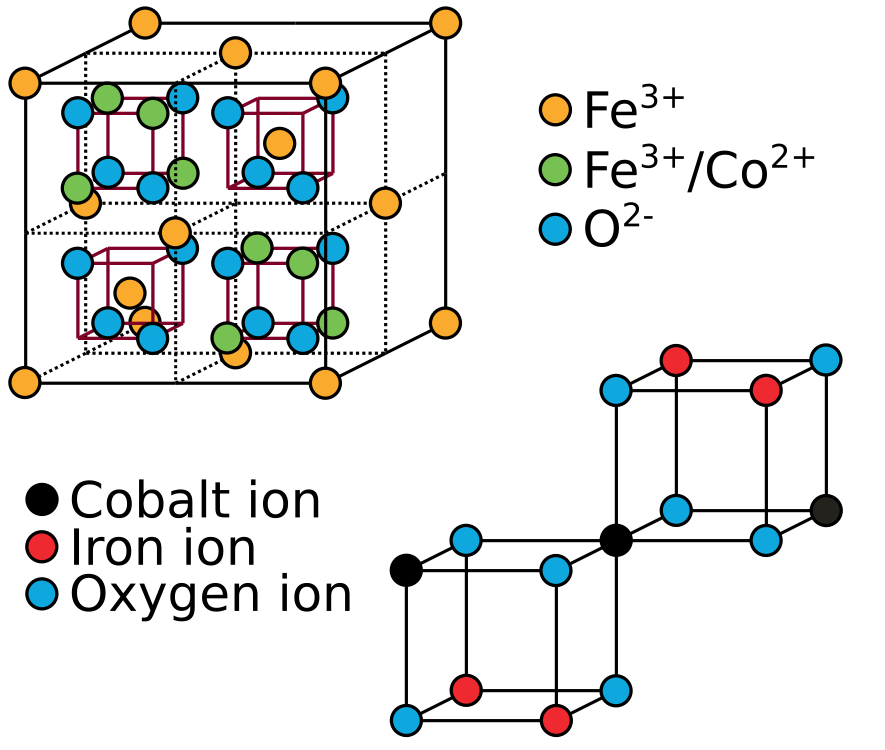
\includegraphics{ferrite_cobaltFerriteStructure}
    \caption{\label{fig:theoreticalBackground:ferrites:cofe2o4Structure}Unit cell of the inverse spinell structure of \ch{CoFe2O4} (upper image) \cite{Sickafus_1999_Struc} and focus on one type of neighborhood of a cobalt ion (lower image) \cite{Tachiki_1960_Origi}. The bordeaux small cubes in the unit cell repeat in the back and are not shown for clarity.}
  \end{figure}

  Similar to magnetite, \ch{CoFe2O4} crystallizes in the inverse spinell structure with the space group $Fd\bar{3}m$.
  Here, the cobalt cations occupy half of the octahedral sites, while the trivalent iron is found on the other half and on the tetrahedral sites, noted by (\ch{Fe^{3+}})[\ch{Co^{2+}Fe^{3+}}]$\ch{O4}$.
  A depiction of the unit cell is shown in \reffig{fig:theoreticalBackground:ferrites:cofe2o4Structure} (upper image), which contains eight formula units.
  The lattice constant for cobalt ferrite is in the order of $a \eq 8.38 \unit{\angstrom}$ \cite{Goldman_1999_Cryst}.
  It can be shown that the magnetic moment and high anisotropy constant of cobalt ferrite is explained broadly by considering the Hamiltonian of a cobalt ion and it's crystalline field as it's depicted in the lower image of \reffig{fig:theoreticalBackground:ferrites:cofe2o4Structure} \cite{Slonczewski_1958_Origi, Tachiki_1960_Origi}.
  From this theory, it is shown that the deduced magnitude and temperature dependence of the cubic anisotropy constant $K_1$ reproduces the experimental result obtained from torque measurements on bulk crystals \cite{Shenker_1957_Magne}
  \begin{align}
    K_1 \eq 1.96 \cdot 10^6 \exp(-1.90 \cdot 10^{-5} T^2) \unit{\frac{J}{m^3}},
  \end{align}
  and the magnetic moment per cobalt ion in cobalt ferrite is derived to be approximately $\mu_\textsf{Co} \eq 3.5 \mu_B$, where reported experimental values are found in the range from $3.3 \mu_B - 3.9 \mu_B$ \cite{Tachiki_1960_Origi}.
  The calculated magnetic moment corresponds to a saturation magnetization of
  \begin{align}
    M_s \eq 8\mu_\textsf{Co}/a^3 \eq 450 \unit{kAm^{-1}}.
  \end{align}

  Detailed studies of the iron atom occupation via M\"ossbauer spectroscopy in a magnetic field show that in actual bulk cobalt ferrite crystals, the structure is a mixed inverse spinell structure, where the iron occupation is not 1:1 in tetrahedral and octahedral positions, but depending on the sample preparation, more iron atoms can shift to the octahedral positions and thus cobalt atoms also occupy the tetrahedral interstices \cite{Sawatzky_1968_Catio, Sawatzky_1969_Mossb}.
  In the case of nanoparticular cobalt ferrite, the relative content of cobalt and iron in the spinell structure, as well as the relative occupation of the sites varies broadly depending on the preparation process and the particle size \cite{Muscas_2015_Evolu, Repko_2015_Oleate, Peddis_2008_Spinc} and has to be studied on a case to case basis.
\end{document}